\documentclass[a4paper,12pt,twocolumn]{article}

% Packages
\usepackage{graphicx}
\usepackage{caption} % more customisation options for captions, used for fontsize in figures.

% Making cites superscript
\usepackage[sorting=none]{biblatex}
\DeclareCiteCommand{\supercite}[\mkbibsuperscript]
{\iffieldundef{prenote}
	{}
	{\BibliographyWarning{Ignoring prenote argument}}%
	\iffieldundef{postnote}
	{}
	{\BibliographyWarning{Ignoring postnote argument}}}
{\usebibmacro{citeindex}%
	\bibopenbracket\usebibmacro{cite}\bibclosebracket}
{\supercitedelim}
{}
\let\cite=\supercite

% Adding the bibliography file
\addbibresource{references.bib}

\begin{document}
	
	\begin{titlepage}
		\begin{center}
			
			\thispagestyle{empty}
			
			\Huge{
				\textbf{UCD School Of Physics}
			}
			
			\vspace{1cm}	
			
			
\includegraphics[scale=0.08]{UCDLogo.png}
			
			\vspace{1cm}
			
			\large{
				\textbf{PHYC30170 Physics with Astronomy and Space Science Lab 1; \\
					CCDs and Spectroscopy \\
					\vspace{1cm}
					18/10/2022 \\
					\vspace{1cm}
					Daragh Hollman}
			} \\
			
		\end{center}
	\end{titlepage}
	
	\twocolumn[
	\begin{@twocolumnfalse}
		\begin{abstract}
			The aim of this experiment was to calibrate a CCD for spectroscopy and determine the resolution of a spectrograph. This was done by comparing the emission spectrum of a mercury arc lap to reference values... INSERT RESULTS.
		\end{abstract}
	\end{@twocolumnfalse}
	]
	
	\section{Introduction}
	
	\section{Theory}
		A diffraction grating is used to split incident light into its separate wavelengths. As a diffraction grating is an array of very narrow and evenly spaced slits, the diffraction pattern from each slit interferes such that the light disperses by a angle $\theta$ as described by equation \ref{eq:diffraction}\cite{universityPhysics}.
		\begin{equation}
			n \lambda = d sin\theta
			\label{eq:diffraction}
		\end{equation} where $d$ is the spacing between the slits, $\lambda$ is the wavelength of the incident light, $\theta$ is the angle which the light is diffracted by and $n$ is a positive integer. This process is the primary element of a spectrograph.\\
	
		A spectrograph is an instrument used to measure incoming light and record its spectrum\cite{atnf}. It splits the incoming light based on its wavelength through diffraction. There are five key components to a spectrograph: telescope, slit, collimator, diffraction grating and detector, as shown in figure \ref{fig:spectrograph}. The telescope focuses the incident light on the slit which only allows a small (ideally 1D) slice of the target through\cite{manual}. The light diverges after the slit and so a collimator is used to make the rays parallel again to ensure that all parts of the light hit the grating at the same angle of incidence. The light then hits the grating and is diffracted at an angle according to its wavelength.
		
		\begin{figure}
			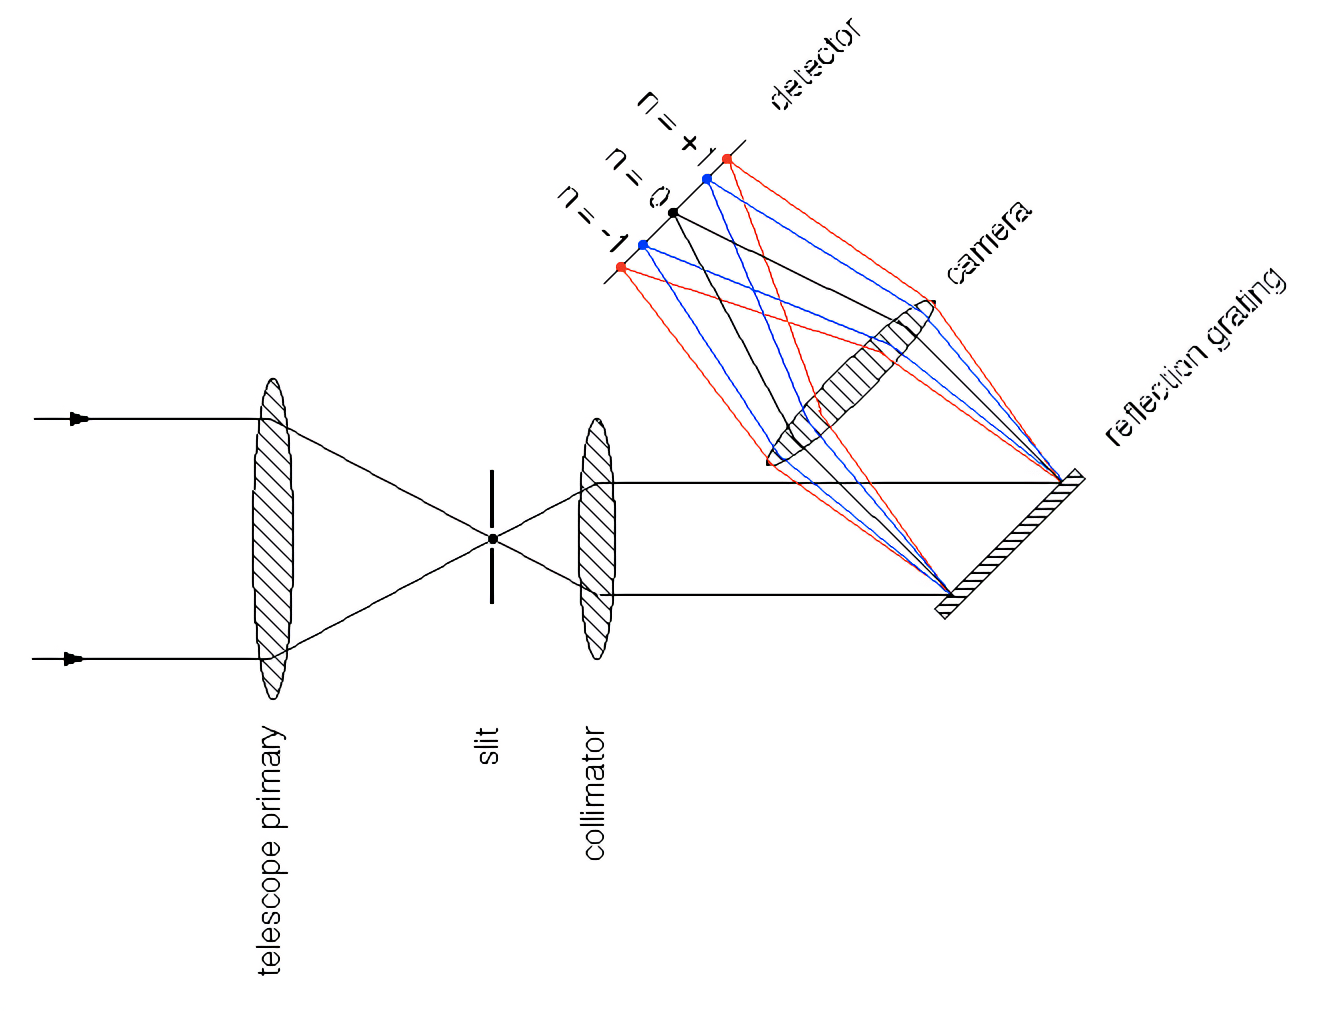
\includegraphics[width=\columnwidth]{spectrograph_refl-transformed.png}
			\captionsetup{font=scriptsize}
			\caption{Diagram of a sample spectrograph setup. The primary lens focuses the incident light through a slit. The collimator makes the rays parallel as they diffract off of the reflection grating. A last lens focuses the rays on the detector.}
			\label{fig:spectrograph}
		\end{figure}
	
		Diffraction grating and equation + figure, what is the spectrograph setup, arc lamps + emission lines
	
	\section{Methodology}
		\subsection{Apparatus}
			Photo of experimental setup + focal lengths of all pieces, Atik 314L+ CCD
	
		\subsection{Determining the Readnoise and the Gain}
		
		\subsection{Wavelength Calibration}
	
		\subsection{Determining the Resolution of the Spectrograph}
	
	\section{Results and Analysis}
	
	\section{Conclusion}
	
	\printbibliography
\end{document}